\section{Bug Reporting in Open Source Projects}


%The problem is real, i.e., there are repos that have more BRs than they can manage. How many BRs arrive at the most popular repos (is the traffic bursty)? how many lack OB/EB/S2R from these?
The overall trend in software development in recent years is towards increased
speed of development and delivery. There are nowadays numerous projects on popular
public software collaboration platforms like GitHub that have large development
teams and user communities. Many of these projects experience significant
bug reporting traffic. Figure~\ref{fig:repo_activity} shows the issue creation
frequency for a selection of ten GitHub repositories that are currently active
with a high numbers of commits and developers. Three of these repositories have
a median of over 40 issues created daily, where most of them are bug reports reported by
GitHub identities that have not contributed to the project (i.e., users). In addition,
the same three projects exhibit high variance in daily issue creation, likely indicative
of bursty and hard to predict bug reporting activity. This is a
considerable burden for bug triagers and it motivates the need for the type of work
as described in this paper, which intends to make bug triage more efficient and less of
a burden for project maintainers.

\begin{figure}[t]
\centering
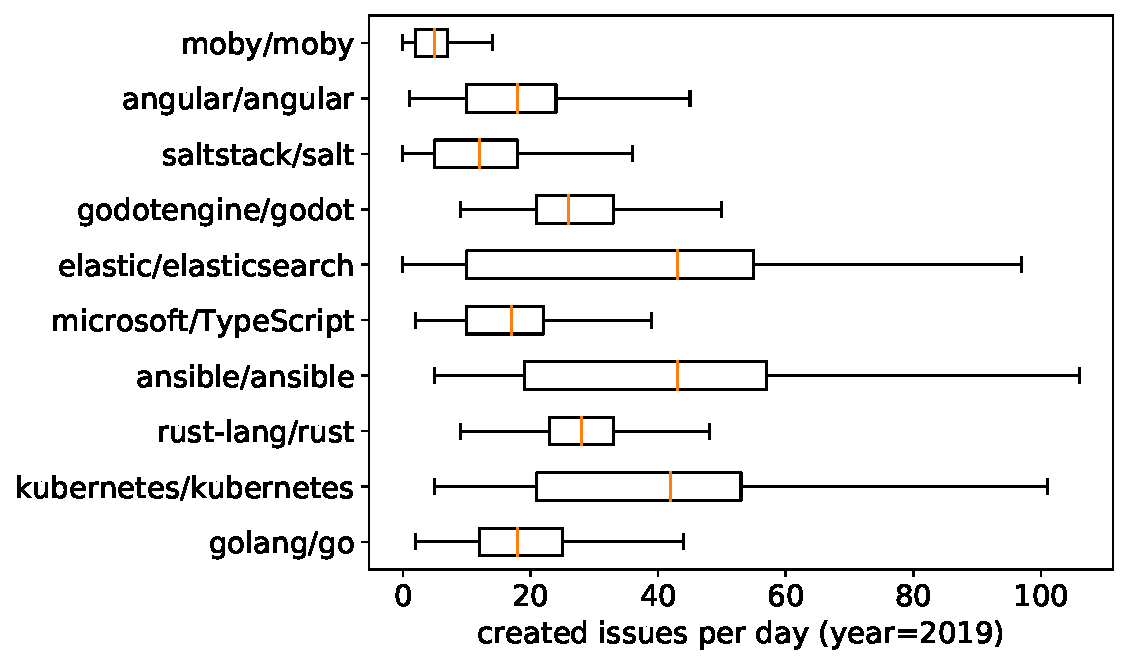
\includegraphics[width=0.99\linewidth]{figures/popular_repos.pdf}
\caption{Daily issue creation activity in 2019 for a selection of ten highly active
(by number of commits) repositories on GitHub.}
\label{fig:repo_activity}
\end{figure}



The preconditions are present, i.e., there are a lot of follow-up questions on GitHub -- we could
use the same set of 10 repos to show this.




Motivate the value of the answer as a way of ranking by finding a follow-up question.
